\documentclass{beamer}

\usepackage{animate}
\usepackage{xcolor}
\usepackage{subfig}
\usepackage{tabularx}

\graphicspath{{./subsections/}}

\defbeamertemplate*{title page}{customized}[1][]
{
  \begin{center}
    \usebeamerfont{institute}\Huge\insertinstitute\par      
  \end{center}
  \centering
  \usebeamerfont{title}\LARGE\inserttitle\par
  \usebeamerfont{subtitle}\Large\insertsubtitle\par
  \bigskip
  \small\usebeamerfont{author}\insertauthor\par
  \usebeamerfont{date}\insertdate\par
}

\institute{Alma Mater Studiorum \\ University of Bologna}
\title{Artificial Intelligence - Deep Learning}
\subtitle{Deep Deblurring project}
\author{Alessandro Dicosola [Matr. 935563]}
\date{}


\begin{document}
    
\begin{frame}
    \titlepage
\end{frame}

% Introduction
\begin{frame}{Introduction}
    \only<1>{
        \framesubtitle{Problem}
        Remove blurring artifact from images
        \begin{itemize}
            \item CIFAR10\cite{cifar10dataset}
            \item REDS\cite{redsdataset}
        \end{itemize}    
    }
    \only<2>{
        \framesubtitle{Hardware}
        \begin{itemize}
            \item CPU: i7-8750H@2.20GHz
            \item GPU: Nvidia GTX 1060 (6 GB)
        \end{itemize}
    }
\end{frame}

\begin{frame}{Autoencoders}
    Networks implemented:
    \begin{itemize}
        \item ResUNet
        \item EDDenseNet
        \item CAESSC
        \item SRNDeblur
    \end{itemize}
\end{frame}
% ======================================= RESUNET ===================================
\begin{frame}{Autoencoders - ResUNet\cite{unet}\cite{resnet}}
    \only<1>{
        \framesubtitle{Architecture}
        \begin{columns}[T]
            \begin{column}{.70\paperwidth}
                \begin{figure}
                    \centering
                    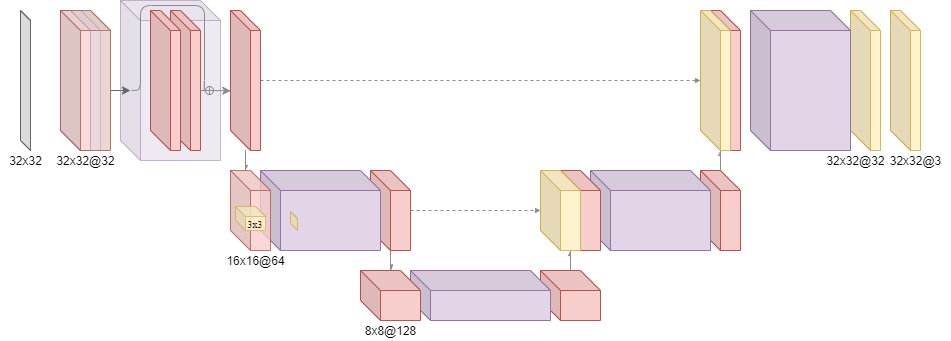
\includegraphics[width=0.70\paperwidth,keepaspectratio]{resunet/resunet.png}
                \end{figure}                                    
            \end{column}
            \begin{column}{.30\paperwidth}
                \begin{itemize}
                    \item The backbone is a UNet architecture
                    \item Use of ResBlock at each level improves the flow of the information
                    \item $\textnormal{Conv} \rightarrow BN \rightarrow ReLU$
                    \item Conv2DTranspose at the end for learning additional information 
                \end{itemize}
            \end{column}
        \end{columns}
    }

    \only<2>{
        \framesubtitle{Results}
        \centering
        \begin{columns}
            \begin{column}[c]{0.45\paperwidth}
                \begin{figure}
                    \centering
                    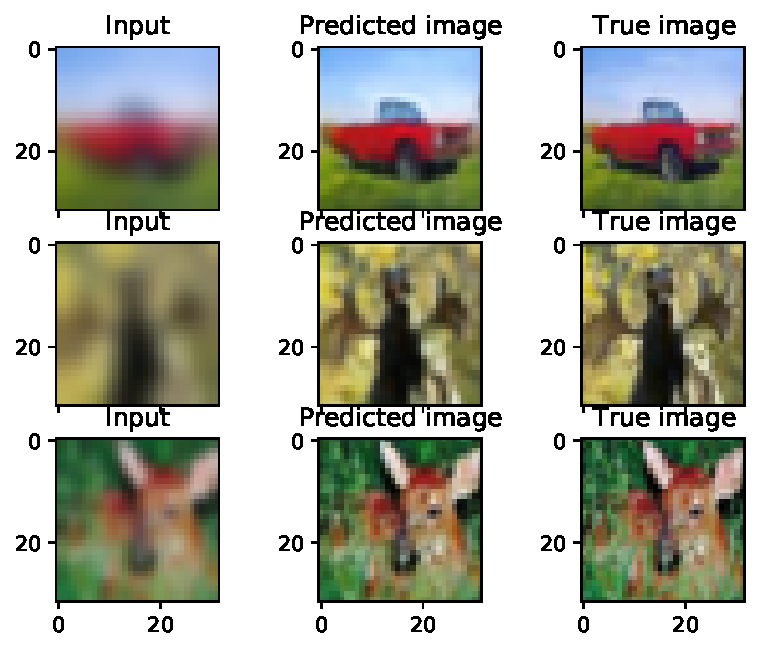
\includegraphics[width=0.45\paperwidth,keepaspectratio]{resunet/resunet1test.pdf}
                    \caption{ResUNet1}
                \end{figure}                        
            \end{column}
            \begin{column}[c]{0.45\paperwidth}
                \begin{figure}
                    \centering
                    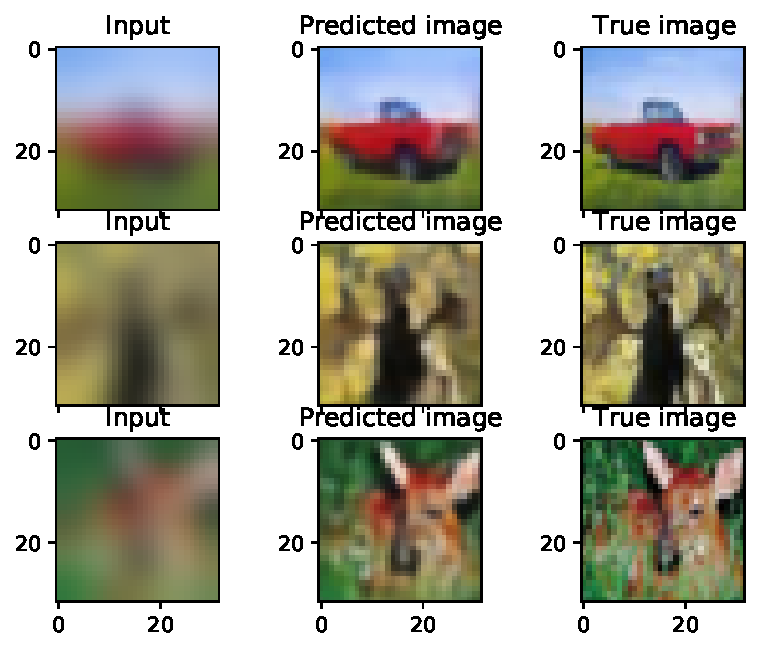
\includegraphics[width=0.45\paperwidth,keepaspectratio]{resunet/resunet3test.pdf}
                    \caption{ResUNet3}
                \end{figure}                        
            \end{column}
        \end{columns}
        \begin{center}
            \tiny
            \begin{tabularx}{0.5\columnwidth}{XXXX}
                \centering
                number of ResBlock & MSE & PSNR & SSIM \\
                1 & 0.0018 & 28.49 & 0.930 \\
                3 & 0.0016 & 29.03 & 0.935
            \end{tabularx}                
        \end{center}
    }
\end{frame}

% ======================================= EDDenseNet ================================
\begin{frame}{Autoencoders - EDDenseNet\cite{densenet}}
    \only<1>{
        \framesubtitle{Architecture}
        \begin{columns}
            \begin{column}[c]{.70\paperwidth}
                \begin{figure}
                    \centering
                    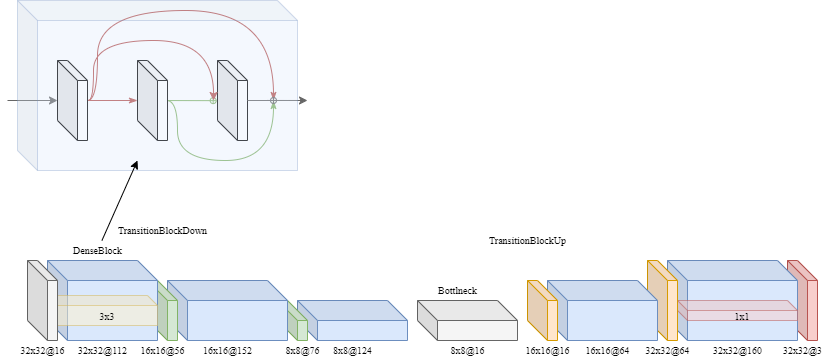
\includegraphics[width=0.70\paperwidth,keepaspectratio]{densenet/densenet.png}
                \end{figure}                                    
            \end{column}
            \begin{column}[c]{.30\paperwidth}
                \begin{itemize}
                    \item Encoder-Decoder architecture
                    \item Use of DenseBlock
                    \item $\textnormal{Conv} \rightarrow BN \rightarrow ReLU$
                    \item Conv2DTranspose at the end
                \end{itemize}
            \end{column}
        \end{columns}
    }
    \only<2>{
        \framesubtitle{Results}
        \begin{columns}
            \begin{column}[c]{\paperwidth}
                \begin{figure}
                    \centering
                    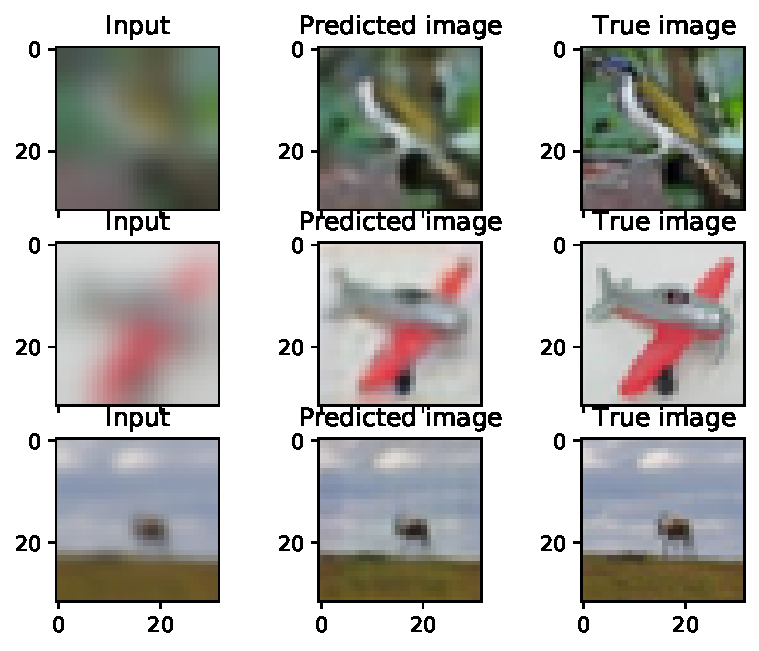
\includegraphics[width=.50\paperwidth,keepaspectratio]{densenet/test.pdf}
                \end{figure}                        
            \end{column}            
        \end{columns}
        \begin{center}
            \tiny
            \begin{tabularx}{0.5\columnwidth}{X|XXX}
                \centering
                kernel type & MSE & PSNR & SSIM \\
                \hline
                gaussian & 0.0021 & 27.62 & 0.90
            \end{tabularx}
        \end{center}
    }
\end{frame}

% ======================================= CAESSC ================================
% TODO train() evaluate() test()
\begin{frame}{Autoencoders - CAESSC\cite{CAESSC}}
    \only<1>{
        \framesubtitle{Architecture}
        \begin{columns}
            \begin{column}[c]{.70\paperwidth}
                \begin{figure}
                    \centering
                    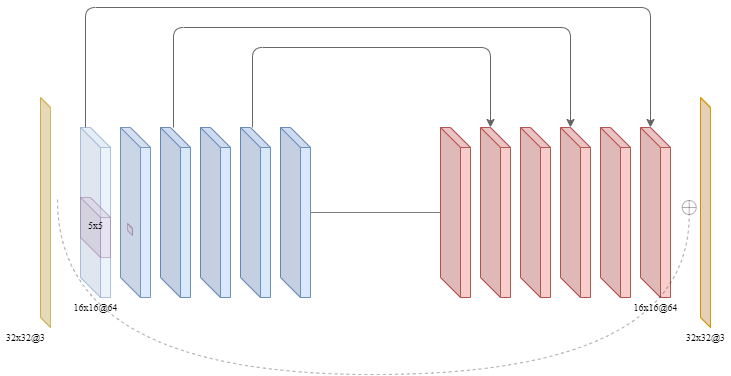
\includegraphics[width=0.70\paperwidth,keepaspectratio]{caessc/caessc.png}
                \end{figure}                                    
            \end{column}
            \begin{column}[c]{.30\paperwidth}
                \begin{itemize}
                    \item Simple structure
                    \item Use of symmetric skip connections between with a fixed interval
                    \item Use of highway skip connection improve the outcome
                \end{itemize}
            \end{column}
        \end{columns}
    }
    \only<2>{
        \begin{columns}
            \begin{column}[c]{0.30\paperwidth}
                \begin{figure}
                    \centering
                    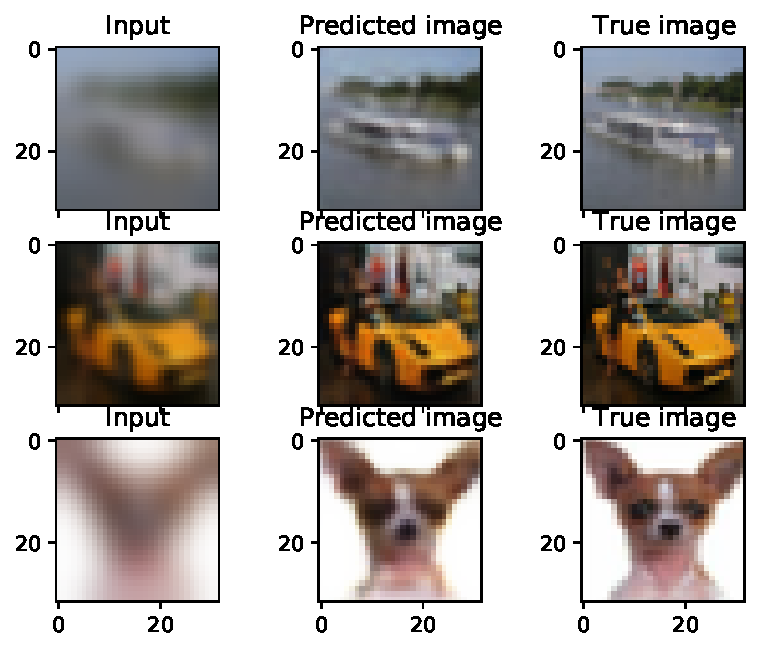
\includegraphics[width=0.30\paperwidth,keepaspectratio]{caessc/d16_f128.pdf}
                    \caption{CAESSC with depth=16 and filters=128}
                \end{figure}
            \end{column}
            \begin{column}[c]{0.30\paperwidth}
                \begin{figure}
                    \centering
                    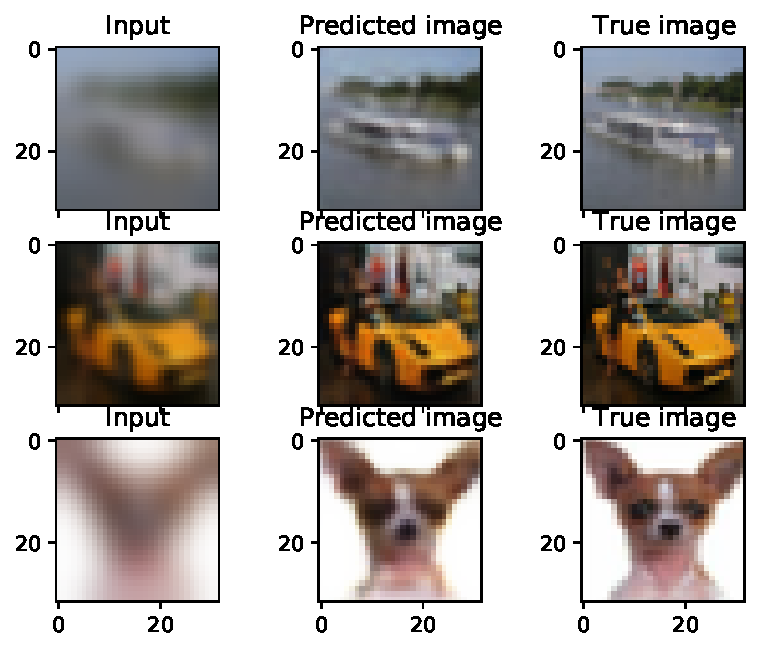
\includegraphics[width=0.30\paperwidth,keepaspectratio]{caessc/d16_f128.pdf}
                    \caption{CAESSC with depth=16 and filters=128}
                \end{figure}
            \end{column}
            \begin{column}[c]{0.30\paperwidth}
                \begin{figure}
                    \centering
                    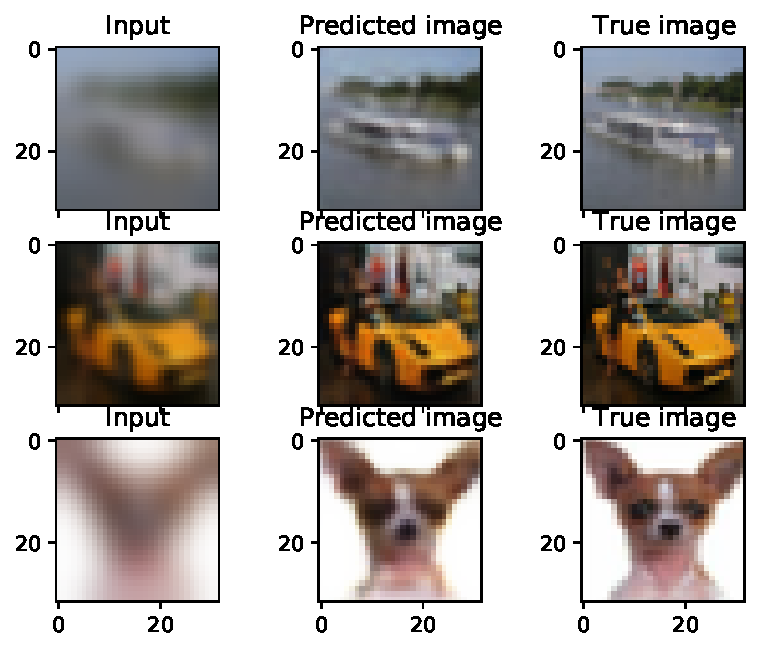
\includegraphics[width=0.30\paperwidth,keepaspectratio]{caessc/d16_f128.pdf}
                    \caption{CAESSC with depth=16 and filters=128}
                \end{figure}
            \end{column}
        \end{columns}
    }
\end{frame}

% ======================================= SRNDeblur ================================
\begin{frame}{Autoencoders - SRNDeblur\cite{SRN-DeblurNet}}
    \only<1>{
        \framesubtitle{Architecture}
        \begin{columns}
            \begin{column}[c]{0.45\paperwidth}
                \begin{figure}
                    \centering
                    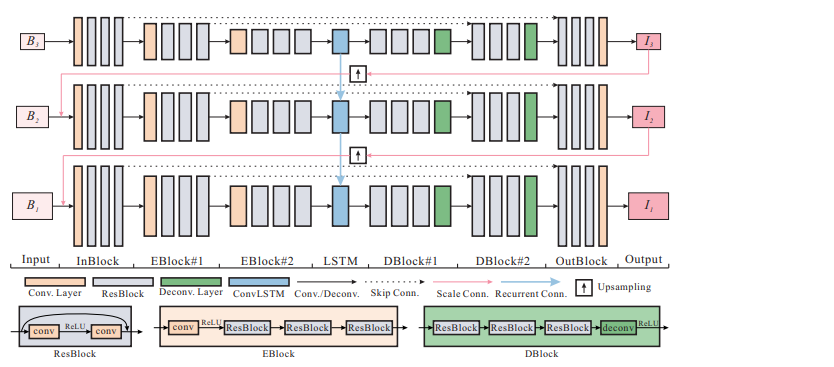
\includegraphics[width=0.60\paperwidth,keepaspectratio]{srndeblur/model.png}
                \end{figure}                                    
            \end{column}
            \begin{column}[c]{.45\paperwidth}
                \begin{itemize}
                    \item FCNN
                    \item Use of Blocks
                    \item Encoder-Decoder architecture
                    \item ResBlocks and skip connections
                    \item Multi-Scale network
                    \item Recurrent layer
                \end{itemize}
            \end{column}
        \end{columns}
    }
    \only<2>{
        \framesubtitle{Training}
        \begin{columns}
            \begin{column}[c]{0.35\paperwidth}
                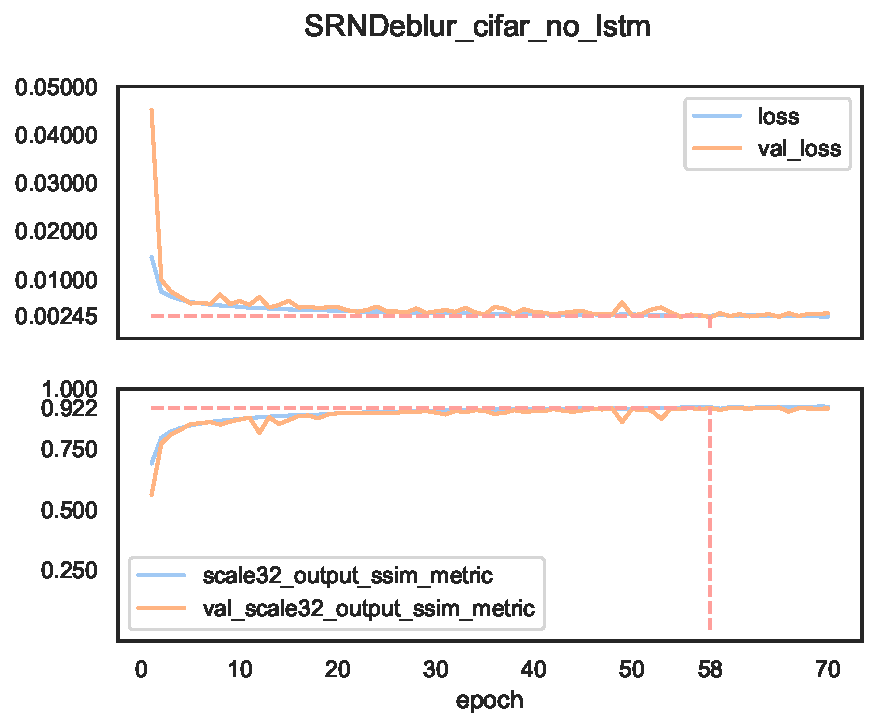
\includegraphics[height=0.3\paperheight,keepaspectratio]{srndeblur/plot_history_SRNDeblur_cifar_no_lstm.pdf}
                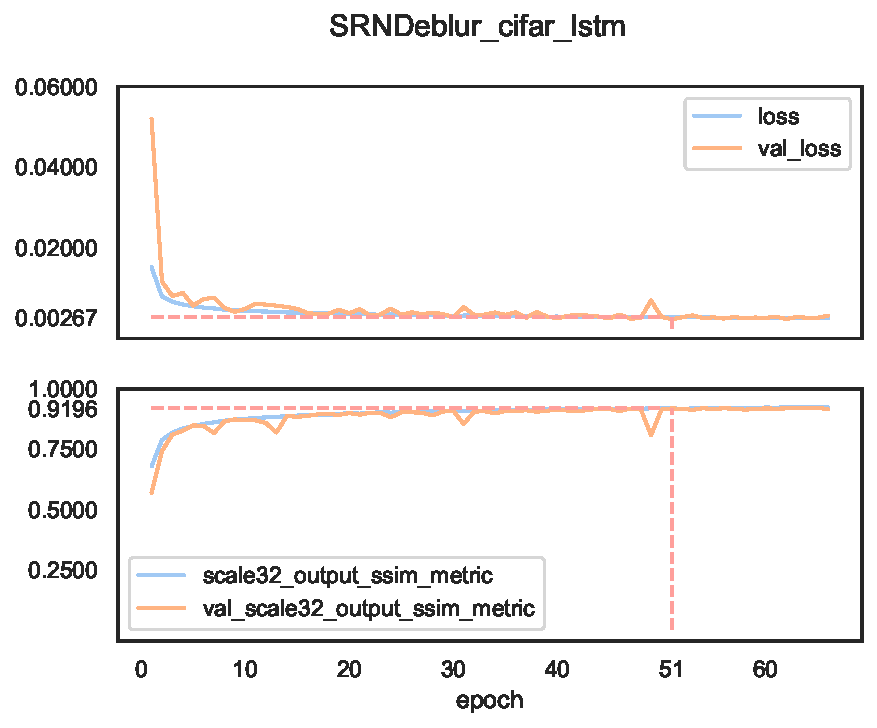
\includegraphics[width=0.3\paperheight,keepaspectratio]{srndeblur/plot_history_SRNDeblur_cifar_lstm.pdf}
                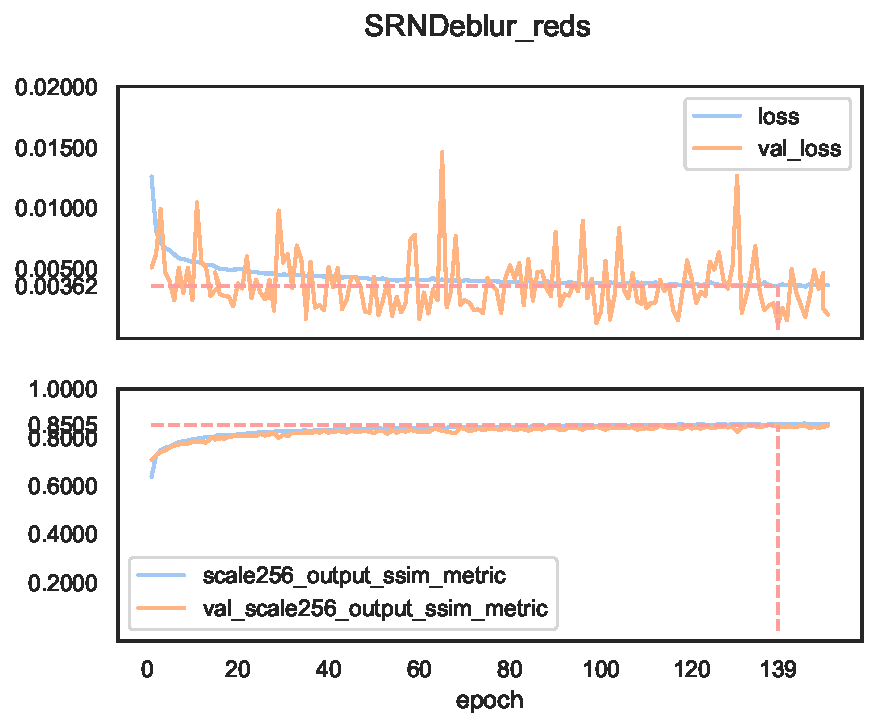
\includegraphics[width=0.3\paperheight,keepaspectratio]{srndeblur/plot_history_SRNDeblur_reds.pdf}
            \end{column}
            \begin{column}[c]{0.50\paperwidth}
                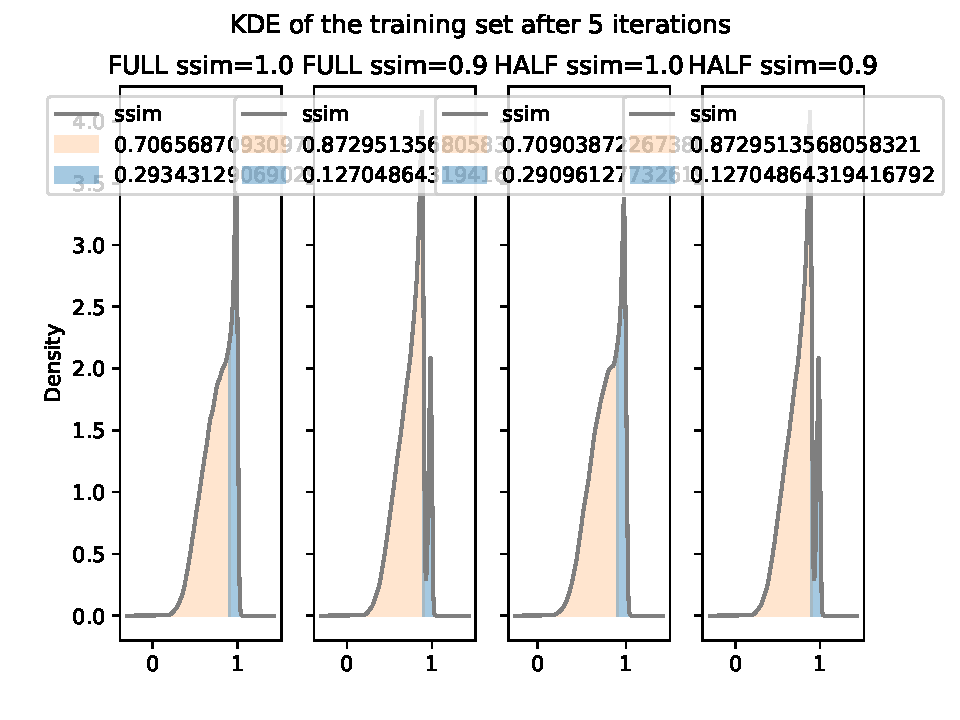
\includegraphics[width=0.45\paperwidth,keepaspectratio]{srndeblur/kde.pdf}
            \end{column}
        \end{columns}

    }

    \only<3>{
        \framesubtitle{Results}
        \begin{figure}
            \animategraphics[autoplay,loop,width=0.53\textwidth,keepaspectratio]{1}{./subsections/srndeblur/gif/frame_}{0}{9}
            \caption{Test image generated by \textcolor{orange}{SRNDeblur\_cifar} network}
        \end{figure}
        \begin{center}
            \tiny
            \begin{tabularx}{0.5\columnwidth}{XXXX}
                CIFAR10 network & MSE & PSNR & SSIM \\
                \hline
                \textnormal{Without LSTM} & 0.00175 & 29.23 & 0.9225 \\
                \textnormal{With LSTM} & 0.00174 & 29.38 & 0.9188 \\
                \hline
            \end{tabularx}                
        \end{center}
    }
    \only<4>{
        \framesubtitle{Results}
        \begin{figure}
            \centering
            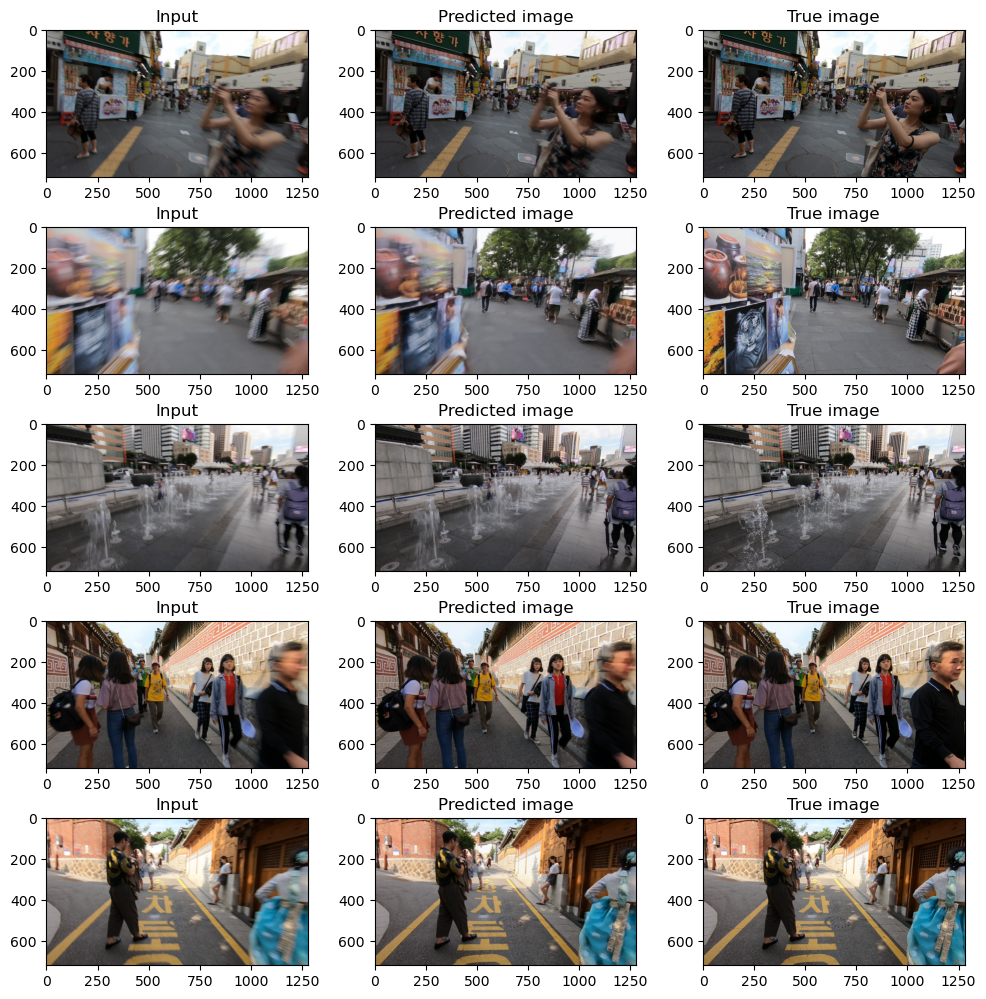
\includegraphics[height=0.57\textheight,keepaspectratio]{srndeblur/test.png}
            \caption{High resolution test image generated by \textcolor{orange}{SRNDeblur\_reds} network.}
        \end{figure}
        
        \begin{center}
            \tiny
            \begin{tabularx}{0.5\columnwidth}{XXXXXX}
                & \multicolumn{3}{c}{SRNDeblur\_reds} & \multicolumn{2}{c}{SRN-DeblurNet} \\
                dataset & MSE & PSNR & SSIM & PSNR & SSIM \\
                \hline
                REDS & 0.002 & 27.23 & 0.8105 & - & - \\
                GOPro & - & - & - & 30.26 & 0.9342 \\
                \hline            
                \end{tabularx}
        \end{center}
    }
    \only<5>{
        \framesubtitle{Results}
        \begin{figure}
            \centering
            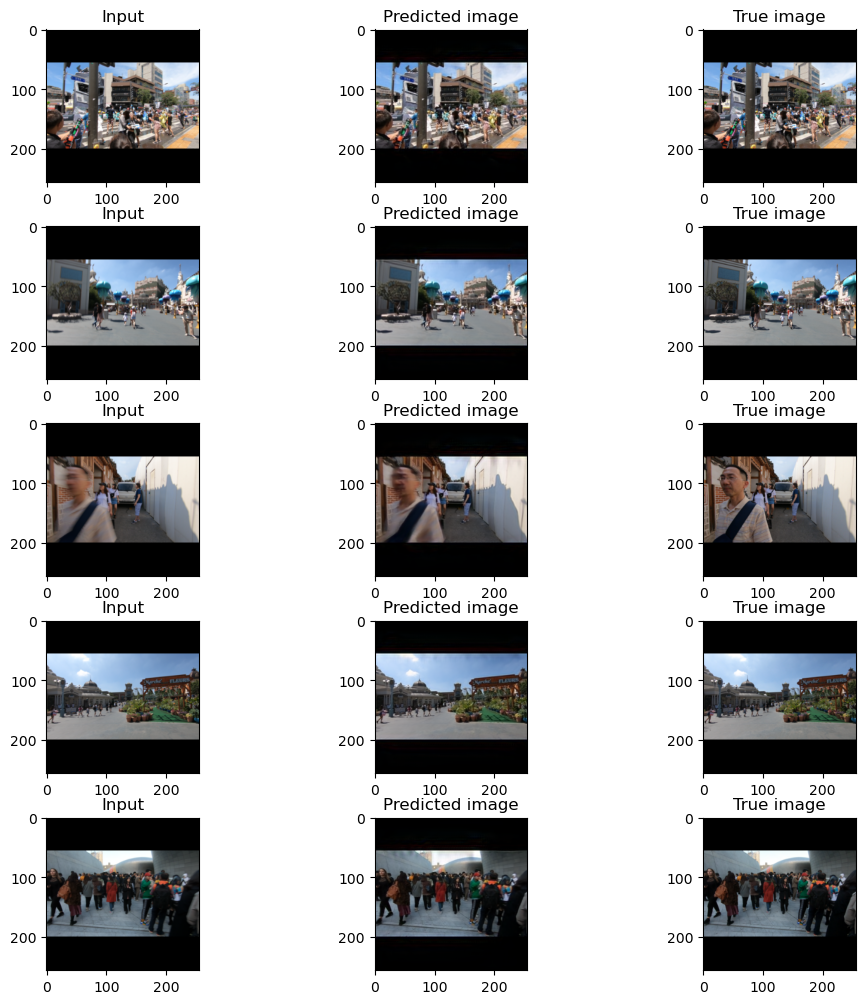
\includegraphics[height=0.75\textheight,keepaspectratio]{srndeblur/test.low_res.png}
            \caption{Low resolution test image generated by \textcolor{orange}{SRNDeblur\_reds} network.}
        \end{figure}
    }

\end{frame}





\begin{frame}{Bibliography}
    \bibliographystyle{ieeetr}
    \bibliography{Report}
\end{frame}
\end{document}
